\documentclass[tikz,border=2pt]{standalone}
\renewcommand{\familydefault}{\sfdefault}
\usetikzlibrary{arrows.meta,calc,positioning}
\tikzset{every picture/.style={line width=1pt, >=Stealth},
         hl/.style={fill=black, fill opacity=0.12, text opacity=1}}
\begin{document}
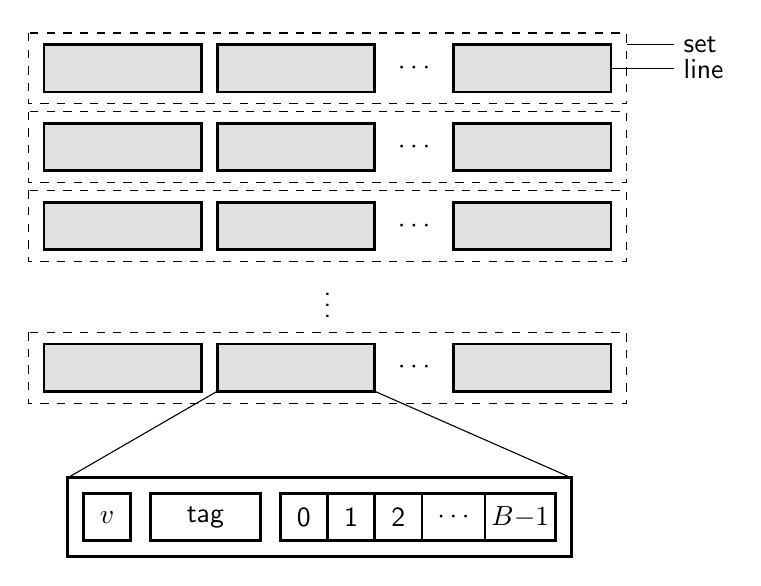
\begin{tikzpicture}[line/.style={draw, hl, minimum width=2cm, minimum height=0.6cm}, set/.style={draw, thin, dashed}]
  % S sets, each with E lines; each line holds a valid bit, a tag, and a block of B bytes.
  \foreach \y in {0, -1, -2, -3.8} {
    \draw[set] (-0.2, \y + 0.45) rectangle (7.4, \y - 0.45);
    \node[line] (a\y) at (1, \y) {};
    \node[line] (b\y) at (3.2, \y) {};
    \node at (4.7, \y) {$\cdots$};
    \node[line] (c\y) at (6.2, \y) {};
  }
  \node at (3.6, -2.9) {$\vdots$};
  \draw[thin] (7.4, 0.3) -- (8, 0.3) node[right] {set};
  \draw[thin] (c0.east) -- (8, 0) node[right] {line};
  % Zoom into one line.
  \draw[thin] (2.2, -4.1) -- (0.3, -5.2);
  \draw[thin] (4.2, -4.1) -- (6.7, -5.2);
  \draw (0.3, -5.2) rectangle (6.7, -6.2);
  \node[draw, minimum size=0.6cm] at (0.8, -5.7) {$v$};
  \node[draw, minimum width=1.4cm, minimum height=0.6cm] at (2.05, -5.7) {tag};
  \foreach \b [count=\i from 0] in {0, 1, 2} \node[draw, minimum size=0.6cm] at (3.3 + 0.6*\i, -5.7) {\b};
  \node[draw, minimum width=0.8cm, minimum height=0.6cm] at (5.2, -5.7) {$\cdots$};
  \node[draw, minimum width=0.9cm, minimum height=0.6cm, inner sep=1pt] at (6.05, -5.7) {$B{-}1$};
\end{tikzpicture}
\end{document}
